\def\year{2020}\relax
%File: formatting-instruction.tex
\documentclass[letterpaper]{article} % DO NOT CHANGE THIS
\usepackage{aaai2020/aaai20}  % DO NOT CHANGE THIS
\usepackage{times}  % DO NOT CHANGE THIS
\usepackage{helvet} % DO NOT CHANGE THIS
\usepackage{courier}  % DO NOT CHANGE THIS
\usepackage[hyphens]{url}  % DO NOT CHANGE THIS
\usepackage{graphicx} % DO NOT CHANGE THIS
\urlstyle{rm} % DO NOT CHANGE THIS
\def\UrlFont{\rm}  % DO NOT CHANGE THIS
\usepackage{graphicx}  % DO NOT CHANGE THIS
\frenchspacing  % DO NOT CHANGE THIS
\setlength{\pdfpagewidth}{8.5in}  % DO NOT CHANGE THIS
\setlength{\pdfpageheight}{11in}  % DO NOT CHANGE THIS
%\nocopyright
%PDF Info Is REQUIRED.
% For /Author, add all authors within the parentheses, separated by commas. No accents or commands.
% For /Title, add Title in Mixed Case. No accents or commands. Retain the parentheses.
 \pdfinfo{
/Title (Wikipedia Path Search)
/Author (Anna Zhang, Cynthia Lee, Regina Wong)
} %Leave this	
% /Title ()
% Put your actual complete title (no codes, scripts, shortcuts, or LaTeX commands) within the parentheses in mixed case
% Leave the space between \Title and the beginning parenthesis alone
% /Author ()
% Put your actual complete list of authors (no codes, scripts, shortcuts, or LaTeX commands) within the parentheses in mixed case. 
% Each author should be only by a comma. If the name contains accents, remove them. If there are any LaTeX commands, 
% remove them. 

% DISALLOWED PACKAGES
% \usepackage{authblk} -- This package is specifically forbidden
% \usepackage{balance} -- This package is specifically forbidden
% \usepackage{caption} -- This package is specifically forbidden
% \usepackage{color (if used in text)
% \usepackage{CJK} -- This package is specifically forbidden
% \usepackage{float} -- This package is specifically forbidden
% \usepackage{flushend} -- This package is specifically forbidden
% \usepackage{fontenc} -- This package is specifically forbidden
% \usepackage{fullpage} -- This package is specifically forbidden
% \usepackage{geometry} -- This package is specifically forbidden
% \usepackage{grffile} -- This package is specifically forbidden
% \usepackage{hyperref} -- This package is specifically forbidden
% \usepackage{navigator} -- This package is specifically forbidden
% (or any other package that embeds links such as navigator or hyperref)
% \indentfirst} -- This package is specifically forbidden
% \layout} -- This package is specifically forbidden
% \multicol} -- This package is specifically forbidden
% \nameref} -- This package is specifically forbidden
% \natbib} -- This package is specifically forbidden -- use the following workaround:
% \usepackage{savetrees} -- This package is specifically forbidden
% \usepackage{setspace} -- This package is specifically forbidden
% \usepackage{stfloats} -- This package is specifically forbidden
% \usepackage{tabu} -- This package is specifically forbidden
% \usepackage{titlesec} -- This package is specifically forbidden
% \usepackage{tocbibind} -- This package is specifically forbidden
% \usepackage{ulem} -- This package is specifically forbidden
% \usepackage{wrapfig} -- This package is specifically forbidden
% DISALLOWED COMMANDS
% \nocopyright -- Your paper will not be published if you use this command
% \addtolength -- This command may not be used
% \balance -- This command may not be used
% \baselinestretch -- Your paper will not be published if you use this command
% \clearpage -- No page breaks of any kind may be used for the final version of your paper
% \columnsep -- This command may not be used
% \newpage -- No page breaks of any kind may be used for the final version of your paper
% \pagebreak -- No page breaks of any kind may be used for the final version of your paperr
% \pagestyle -- This command may not be used
% \tiny -- This is not an acceptable font size.
% \vspace{- -- No negative value may be used in proximity of a caption, figure, table, section, subsection, subsubsection, or reference
% \vskip{- -- No negative value may be used to alter spacing above or below a caption, figure, table, section, subsection, subsubsection, or reference

\setcounter{secnumdepth}{0} %May be changed to 1 or 2 if section numbers are desired.

% The file aaai20.sty is the style file for AAAI Press 
% proceedings, working notes, and technical reports.
%
\setlength\titlebox{2.5in} % If your paper contains an overfull \vbox too high warning at the beginning of the document, use this
% command to correct it. You may not alter the value below 2.5 in
\title{Wikipedia Path Search}
%Your title must be in mixed case, not sentence case. 
% That means all verbs (including short verbs like be, is, using,and go), 
% nouns, adverbs, adjectives should be capitalized, including both words in hyphenated terms, while
% articles, conjunctions, and prepositions are lower case unless they
% directly follow a colon or long dash
\author{Written by\\ \Large \textbf{Anna Zhang, Cynthia Lee, Regina Wong} \\ % All authors must be in the same font size and format. Use \Large and \textbf to achieve this result when breaking a line
% \textsuperscript{\rm 1}Association for the Advancement of Artificial Intelligence\\ %If you have multiple authors and multiple affiliations
% use superscripts in text and roman font to identify them. For example, Sunil Issar,\textsuperscript{\rm 2} J. Scott Penberthy\textsuperscript{\rm 3} George Ferguson,\textsuperscript{\rm 4} Hans Guesgen\textsuperscript{\rm 5}. Note that the comma should be placed BEFORE the superscript for optimum readability
112167606, 111737790, 112329774\\
anna.zhang.2@stonybrook.edu, cynthia.lee.2@stonybrook.edu, regina.wong@stonybrook.edu % email address must be in roman text type, not monospace or sans serif
}
 \begin{document}

\maketitle
\begin{abstract}

The goal of this application is to find one of the shortest
paths to get from one Wikipedia page to another Wikipedia page.
The edges are is determined by hyperlinks on the page. The application will return 
one of the shortest paths using the specified algorithm.

\end{abstract}


\section{Introduction}

The overall objective of our project is to examine different path finding algorithms. Website navigation is important to user experience. When users navigate through a web application, it is intuitive to have relevant pages linked. Wikipedia is a popular website that links sources to other web pages. Many people use Wikipedia for causal research. With more efficient algorithms, it would be easier and faster to search for paths between these pages. Some applications of this problem is website page ranking and user analysis. Page ranking analyzes how popular or important a web page is by ranking it to other web pages. One major application that utilizes page ranking are search engine results. With page ranking, the Wikipedia pages can be examined on which web pages are most frequently visited and the popularity of the links within the page. They can also be examined on how many clicks does it usually take from one user to navigate to another page or which path do users usually take. Other possible analysis can be of how easy it is to find a page and how closely one article term/name relates to another. Analyzing with time can also be done with examining how long it usually takes one user to get to another page as well as what the the fastest way to get from one page to another.\\ 

From the dataset we used, it's sources show that it uses the Floyd-Warshall algorithm. The algorithm calculates all the shortest paths between all pairs of vertices. \\

One issue with the approaches above is the time and space complexity. From the dataset, they used Floyd-Warshall algorithm, which requires at least $O(n^2)$ data for the table and takes $O(n^3)$ for time complexity. The dataset is large with 4604 nodes, 119882 edges, and an average in and out degree of 26.0387. Since the dataset is large, it requires a lot of time and resources. Another issue with this problem is that it is an uninformed search which comes with limitations. Being an uninformed search, it cannot use knowledge for the searching process and cannot utilize many heuristics. There is no way to guarantee that a heuristics can under estimate. Uninformed searches are slower than informed searches because of this.\\

We would turn to algorithms that that only find one path at a time. In addition, we chose algorithms that don't have require a $n$ by $n$ matrix. This would lower the space required since we are only focusing how to get from a to b and ignoring everything else. Only the path from the source to the target is needed. In addition it would take less time, this is because it doesn't have to make more checks to determine if other things fail.\\

The baseline to problem is applying the depth first search (DFS) to the graph. This algorithm doesn't guarantee that it would return the shortest path. However, it is a easy to understand and popular algorithm which is why we chose it as our baseline model. We turned to different methods and improvements to depth first search.\\

Most of our initial ideas at relied on heuristics. We had thought of using BFS with layered detection and/or branch and bound. We had also thought of using best first search, A* with tree adaptive A* or iterative deepening. However, because the problem is an uninformed search, there wasn't a way to define consistent heuristics that wouldn't overestimate the estimated distance. We realized that the problem is an uninformed search and our initial ideas pertained to informed search. With this realization, we were not able to utilize heuristics available to informed searches, and it caused a lot of our initial ideas to be dropped. We then tried to implement the Floyd-Warshall algorithm ourselves. However, that results in a large amount of space needed for the matrix to store the cost of paths and is not efficient. Additionally, we ruled out Dijkstra's algorithm because it also creates a large matrix to store the cost of paths. Our dataset has a large number of nodes and edges which would not make this feasible to implement. If we were to use either Floyd-Warshall or Dijkstra, it would produce a matrix with over 4,600 * 4,600 elements.\\

Outcome:

\begin{enumerate}
  
\item We implemented a Wikipedia path finder to examine the different algorithms for path finding
\item Compared different path finding algorithms for uninformed search
\item Explore algorithms that were discussed in lecture that we didn't do in our assignments
\end{enumerate}

\section{Your Task}

The program takes in the source article name and the target article name from the user via the terminal. In addition, it takes an additional argument which the user can specify a file path to write the output to. The program then would write to an output file the path from $starting\_article$ to $ending\_article$. The output also details the time in millisecond (ms) and the number of nodes explored to calculate that shortest path.


\subsection{Baseline Model(s)}

Our baseline system uses depth first search. Depth first search utilizes a stack to store the nodes that need to be explored. It also contains a list of all the items that were already explored. This guarantees that the traversal does not enter a loop. While the stack isn't empty, the algorithm examines the first node in the stack and then adds it to the explored list. Afterwards, it checks if that node was the target. If it is not, it will add all the children/neighbors of the current node to the stack.

The figure below shows the order of nodes for the graph traversal.

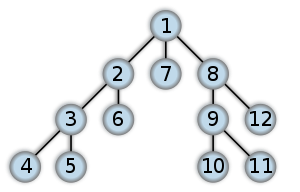
\includegraphics[width=0.35\textwidth]{Images/BFS_tree.png}

\subsection{The Issues}

The main problem with depth first search is that it isn't optimal. In other words, if there is a shorter path with another node, it won't catch it first. This would result in a path that is a longer than the shortest. In the figure below, it shows a case where depth first search isn't optimal. 

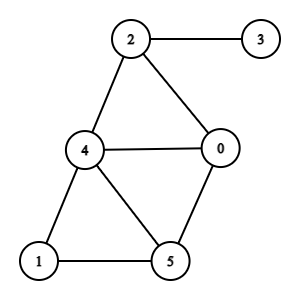
\includegraphics[width=0.30\textwidth]{Images/graph.png}

Suppose that in the figure above, start is 0 and goal is 1 and the list of adjacent are in numerical order. If the program is optimal, it would choose [0, 4, 1] or [0, 5, 1]. Since the adjacent nodes are stored in numerical value, the path returned would be [0, 2, 4, 1]. This is a smaller scale example, but for out dataset that can be a difference of 3 nodes to all 4,604 nodes.

\section{Your Approach}

\subsection{Breadth First Search:}\\
Unlike depth first search, breadth first search is guaranteed to be optimal. That means it will always return the shortest path if the path exists. In the algorithm's code it has a queue, visited list, and parents list. The queue stores node that need to be explored. The visited list stores all the nodes that have been explored to prevent the code from looping and revisiting. While there are elements in the queue, it would check if that node is equal to the target. If not, it will put all the adjacent/neighboring nodes into the queue. The parents list is utilized to return the path that was taken.\\
This guarantees optimality because it makes sure that you check all the nodes of that length before it goes to the next one. 

\subsection{Iterative Deepening Depth First Search:}\\
Iterative deepening depth first search is a combination of depth first search and breadth first search. It takes the good things from both searches. It takes the space efficiency of depth first search and the time complexity of breath first search.\\
Iterative deepening depth first search calls a helper function that recursively calls itself. It checks if there the depth is 0 (Iterative deepening depth first search limits the depth of the search). If not, it goes through all the adjacent/neighboring nodes of the current node that hasn't been visited and then is added to the node of visited. It recursively calls itself for each adjacent node. With each iteration where it does not find a solution, the depth increases by 1. 

\subsection{Bidirectional Search:}\\
For bidirectional search, it utilizes two breadth first searches, one on each ends. One search starts on the source node while the other search starts on the target node. The idea of this search is that both search would have to travel $n/2$ nodes and meet in the middle. Each search has its own queue, visited, and parent variables. For both searches, the queue keeps track of the nodes that will be explored next. Similar to the previous algorithms mentioned, for each search we have an visited list to prevent looping and revisiting.\\
While both queues aren't empty, it would pop elements from their respective queue. If the node element that is popped from the first queue isn't the target or in the other queue, it would add all it's adjacent/neighboring nodes in it's respective queue. The same happens for the second queue.

\section{Evaluation}

State the purpose of your evaluation. How should one evaluate a system for your task. What are the questions to ask?

We evaluated the system based on completeness, time complexity, space complexity and number of nodes expanded. When evaluating search strategies these are taken to account. With completeness we aim to find the shortest possible path. Time complexity, space complexity and number of nodes are used to measure performance/efficiency for speed and resource usage.

\subsection{Dataset Details}

We obtained the dataset from Stanford University's Stanford Network Analysis Project (SNAP) dataset collection. We are working with the Wikipedia navigation paths\footnote{https://snap.stanford.edu/data/wikispeedia.html}\\
This data two files that we utilized. The articles.tsv file includes all the Wikipedia article titles separated by a new line. The links.tsv file includes the edges for the Wikipedia articles, each edge is represented with 2 article names, which represent which one article page linking to another article page. The links are formatted such that the source\_article tab target\_article. Each link is also separated by new line.\\
The dataset has 4604 articles (nodes) and 11,9882 links (edges). There is an average of approximately 26 edges leaving and entering a node on average.

\subsection{Evaluation Measures}

\subsection{Baselines}

We utilized the basic version of depth first search. The worst case time complexity is $O(V + E) = O (b^d)$ and worst case space complexity is $O(V) = O(bd)$. Where $V$ is the number of nodes visited, $E$ is the number of edges, $b$ is the branching factor (~26), $d$ is the depth of the node.

\subsection{Results}

Main results that compares your ideas to the baselines.
What does this result tell you?\\

Complexity for different path finding algorithms\\

    \begin{tabular}{l|l|l}
        & Worst-Case time & Worst-Case space\\
        \hline
        DFS &$O(|V| + |E|)$ & $O(|V|)$\\
        BFS &$O(b^d)$ & $O(b^d)$\\
        IDDFS&$O(b^d)$& $O(d)$\\
        Bidirectional &$O(b^d/2)$ & $O(b^d)$\\
    \end{tabular}
    
DFS vs BFS

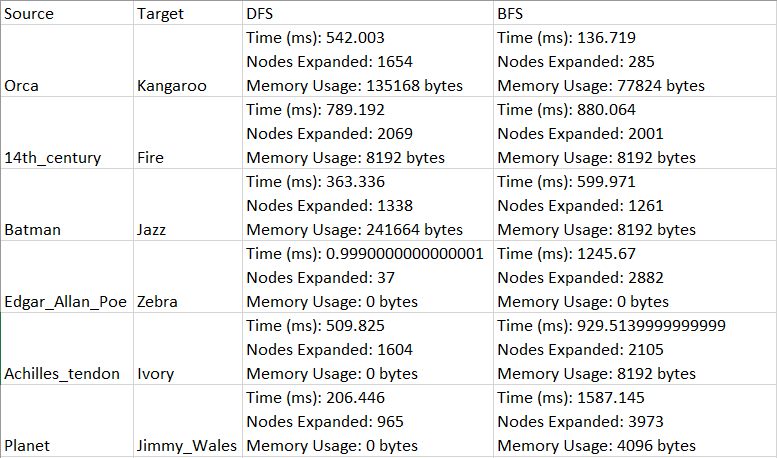
\includegraphics[width=0.5\textwidth]{Images/BFS.png}

DFS VS Deepening

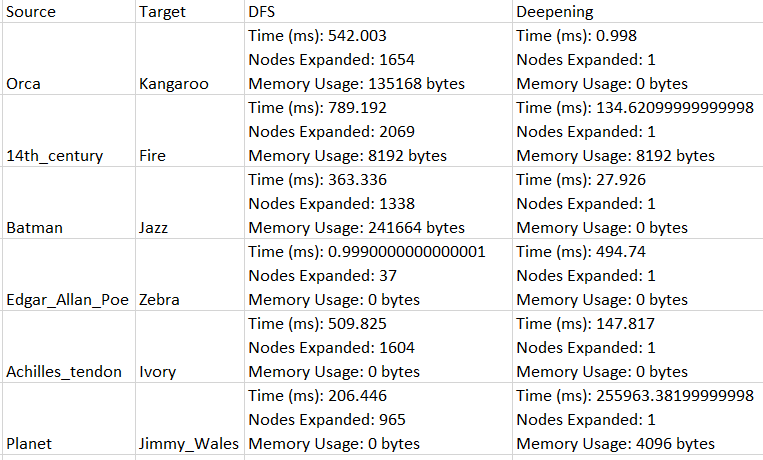
\includegraphics[width=0.5\textwidth]{Images/Deepening.png}

BFS vs Bidirectional

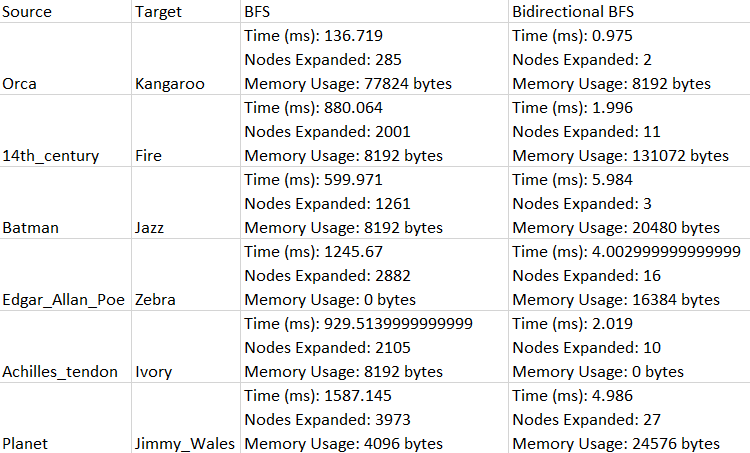
\includegraphics[width=0.5\textwidth]{Images/BidirectionalBFS.png}



\subsection{Analysis}

Heuristics were not able to work with this uninformed search problem, which is mentioned in the introduction for paragraph 5. For error analysis, the ordering of the node's neighbors will effect the node choices in the path. For DFS since the algorithm is not optimal, the code will encounter infinite loops or an extremely long path where it will get stuck.

\subsection{Code}

Github: https://github.com/AnnaZhang2/AI\_Final\_Project\\
Note: You cannnot copy and paste the link above, it removes the underscores

\section{Conclusions}

What we learned form this project is the different algorithms that can be utilized for an uninformed search. DFS can be improved with iterative deepening. BFS can be improved with bidirectional search. From the results it illustrates the pros and cons of trade offs between the algorithms.

\begin{thebibliography}{10}

\bibitem{Bidirectional1} Bidirectional Search.,
\\\texttt{https://en.wikipedia.org/wiki/\allowbreak Bidirectional\_search}

\bibitem{Bidirectional2} Bidirectional Search.,
\\\texttt{http://planning.cs.uiuc.edu/node50.html}

\bibitem{FloydWarshall} Finding Shortest Path between Any Two Nodes Using Floyd Warshall Algorithm.,
\\\texttt{www.geeksforgeeks.org/finding-shortest-\allowbreak path-between-any-two-nodes-using-floyd\allowbreak-warshall-algorithm/}

\bibitem{Iterative} Iterative Deepening Depth-First Search.,
\\\texttt{en.wikipedia.org/wiki/Iterative\_deepening\allowbreak\_depth-first\_search.}

\bibitem{Network} Ladd, John R., et al. Exploring and Analyzing Network Data with Python., Programming Historian, 23 Aug. 2017,
\\\texttt{programminghistorian.org/en/lessons/\allowbreak exploring-and-analyzing-network-data-\allowbreak with-python\#reading-files-importing- \allowbreak data.}

\bibitem{Human} Robert West and Jure Leskovec:
     Human Wayfinding in Information Networks.
     21st International World Wide Web Conference (WWW), 2012.
     
\bibitem{} Robert West, Joelle Pineau, and Doina Precup:
     : An Online Game for Inferring Semantic Distances between Concepts.
     21st International Joint Conference on Artificial Intelligence (IJCAI), 2009.
\\\texttt{http://infolab.stanford.edu/$\sim$west1/pubs/\allowbreak West-Pineau-Precup\_IJCAI-09.pdf}

\bibitem{NetworkX}“Tutorial.” Tutorial - NetworkX 2.5 Documentation, 22 Aug. 2020, \\\texttt{networkx.org/documentation/stable/\allowbreak tutorial.html}

\end{thebibliography}


\end{document}
